\begin{figure}[htbp]
\centering
\begin{tikzpicture}[x=1cm,y=1cm]
\node[anchor=south west,inner sep=0] at (0,0) {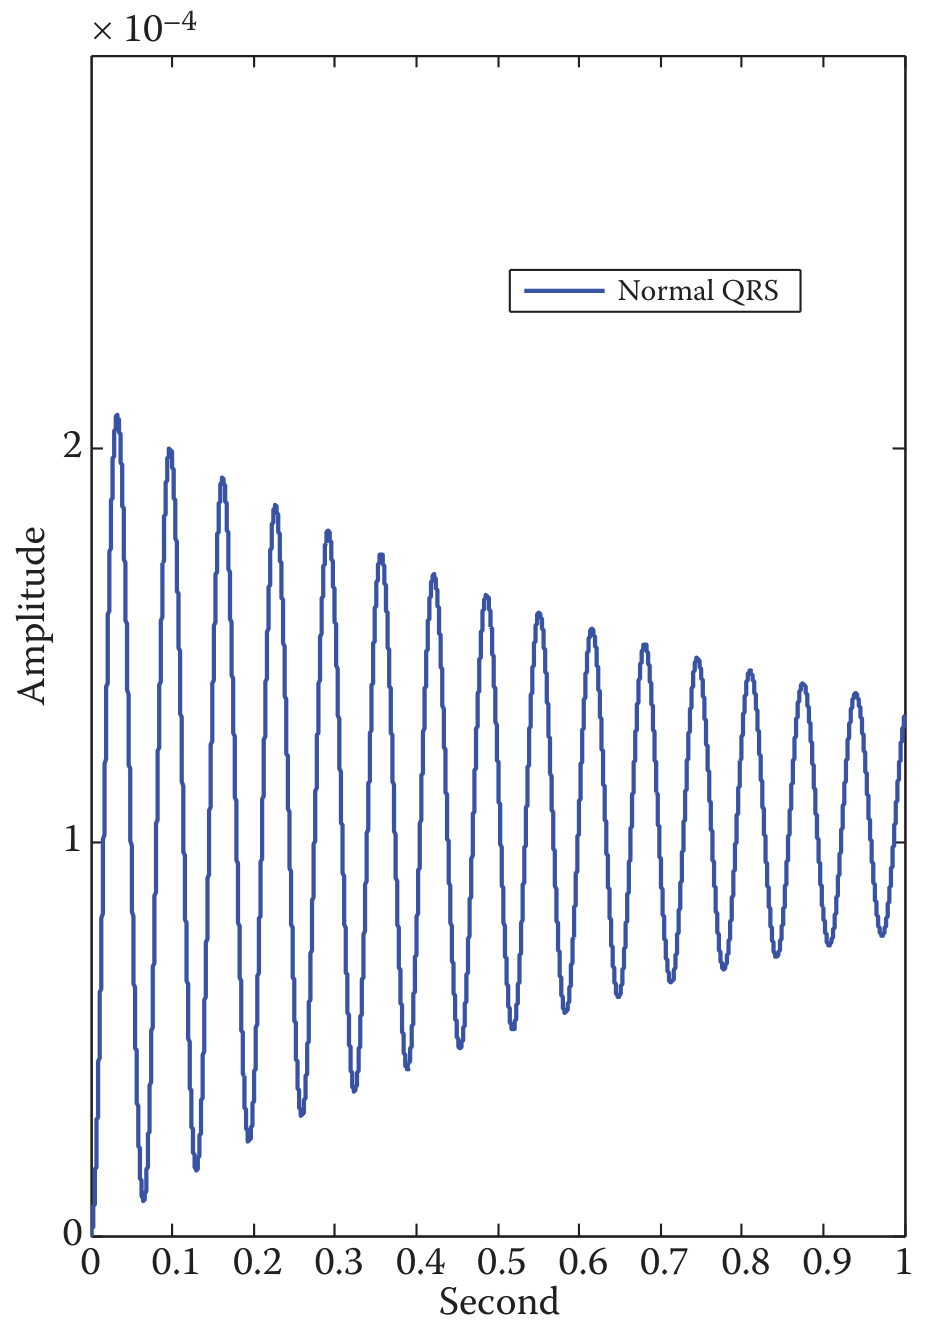
\includegraphics[width=9.0cm]{figures/ch03_fig07_data.png}};
\fill[white] (5.9838,9.9924) rectangle (7.7595,10.3427);
\fill[white] (4.2377,0.0854) rectangle (5.4792,0.5232);
\node[font=\scriptsize,rotate=0,inner sep=0] at (4.8585,0.3043) {时间（秒）};
\fill[white] (0.1094,6.0974) rectangle (0.5570,7.8916);
\node[font=\scriptsize,rotate=90,inner sep=0] at (0.3332,6.9945) {振幅};
\node[font=\scriptsize,rotate=0,inner sep=0] at (6.7949,10.1397) {正常 QRS};
\end{tikzpicture}
\origfig{7}{正常 QRS 波群所对应心脏系统的单位冲激响应曲线。}
\label{fig:ch03-07}
\end{figure}
